\sectioncounter{13}
  \section{利用导数研究函数的单调性}

  \subsection{知识梳理}
  对函数 $f(x)$, 若其图象在点 $(x_0,f(x_0))$ 附近单调递增, 
  不妨在 $x_0$ 附近取 $x_1>x_0$, 则 $f(x_1)>f(x_0)$. 再由导数的定义,
  \[f'(x_0)= \lim_{x_1\to x_0} \frac{f(x_1)-f(x_0)}{x_1-x_0}\geqslant 0.\]
  同样可以说明, 若 $f(x)$ 的图象在点 $(x_0,f(x_0))$ 附近单调递增,
  则 $f'(x_0)\leqslant 0$. 把两个结论写到一起就是
  \begin{align*}
    &f'(x_0)\geqslant 0\iff \text{$f(x)$ 在点 $x=x_0$ 附近单调递增},\\
    &f'(x_0)\leqslant 0\iff \text{$f(x)$ 在点 $x=x_0$ 附近单调递减},
  \end{align*}
  即导数的正负号决定了函数的单调性. 若在 $(a,b)$ 上恒有 $f'(x)>0$, 
  则 $(a,b)$ 是 $f(x)$ 的单调递增区间. 类似的, 若在 $(a,b)$ 上恒有 $f'(x)<0$, 
  则 $(a,b)$ 是 $f(x)$ 的单调递减区间. 下面举例说明利用导数确定函数的单调性的步骤. 
  
  设函数 $f(x)=\mathrm{e}^x -x$, 求导得 $f'(x)= \mathrm{e}^x-1$. 
  先求出导数正负号的分界点, 即导数的零点. 令 $f'(x)=0$ 知所求零点为 $x=0$. 
  再对函数单调性列表如下:
  \begin{center}
    \small
    \begin{tabular}{c|ccc}
      $x$  & $(-\infty,0)$ & 0 & $(0,+\infty)$ \\
      \hline
      $f'(x)$ & $-$ & 0 & $+$ \\
      $f(x)$ & $\searrow$ & 最小值 & $\nearrow$
    \end{tabular}
  \end{center}
  从上述过程可知, $f(x)\geqslant f(0)$ 即 $\mathrm{e}^x\geqslant x+1$ 恒成立,
  \mymarginpar{利用 $\mathrm{e}^x\geqslant x+1$ 可以证明当 $a>0$ 且 $x$ 充分大时, $\mathrm{e}^x> ax$ 或 $\mathrm{e}^x> x^a$, 等价地, $ax>\ln x$ 或 $x^a>\ln x$.}
  表明可以利用导数证明不等式. 
  
  在判断导数的正负号时一般可以借助常见函数的图象.
  但有时导数不是常见的函数, 可能需要对导数再次求导, 以确定导数的增减性并作出其大致图象,
  进而判断导数的正负号. 另外, 求单调区间时也应先确定函数的自然定义域.
  

  \lianxi
  \begin{exercise}
    求函数 $f(x)=5x^2 -2x$ 的单调递增区间.
  \end{exercise}

  \beginsolution
    $f'(x)=10x-2\leqslant 0$, 则 $x\leqslant \frac15$.
  \endsolution
  
  \begin{exercise}
    求函数 $y=x^2-\ln x$ 的单调递减区间.
  \end{exercise}

  \beginsolution
    $x>0$ 且 $y'=2x-\frac1x\leqslant 0$, 
    \mymarginpar{$\ln x$ 中, $x>0$.}
    则 $0<x\leqslant \frac{\sqrt2}2$.
  \endsolution
  
  \begin{exercise}
    若 $f(x)=\mathrm{e}^x -ax$ 在 $(1,+\infty)$ 上单调递增,
    求 $a$ 的取值范围.
  \end{exercise}

  \beginsolution
    $f'(x)=\mathrm{e}^x-a\geqslant 0$ 在 $(1,+\infty)$ 上恒成立, 由 $f'(x)$ 在 $(1,+\infty)$ 上 $\nearrow$ 知 $f'(1)\geqslant 0$, 即 $a\leqslant \mathrm{e}$.
    
    \varexercise 若 $f(x)=\mathrm{e}^x -ax$ 在 $(-\infty,1)$ 上单调递减,
    求 $a$ 的取值范围.
    
    $f'(x)=\mathrm{e}^x-a\leqslant 0$ 在 $(-\infty,1)$ 上恒成立, 由 $f'(x)$ 在 $(-\infty,1)$ 上 $\searrow$ 知 $f'(1)\leqslant 0$, 即 $a\geqslant \mathrm{e}$.
    
    \varexercise 若 $f(x)=\mathrm{e}^x -ax$ 在 $(1,+\infty)$ 上是单调的,
    求 $a$ 的取值范围.
    
    (1) $f'(x)=\mathrm{e}^x-a\geqslant 0$ 在 $(1,+\infty)$ 上恒成立, 则 $a\leqslant \mathrm{e}$.
    
    (2) $f'(x)=\mathrm{e}^x-a\leqslant 0$ 在 $(1,+\infty)$ 上恒成立, 则 $a\geqslant \mathrm{e}^x$, 不可能.
  \endsolution
  
  \begin{exercise}
    若 $f(x)=\mathrm{e}^x -ax\geqslant 1$ 在 $\mathbb{R}$ 上恒成立,
    求 $a$ 的取值范围.
  \end{exercise}

  \beginsolution
    由 $f(0)=1$ 知 $f(x)\geqslant f(0)$ $\mathbb{R}$ 上恒成立, 所以 $f(0)$ 为 $f(x)$ 的最小值, $f'(0)=0$. 由 $f'(x)=\mathrm{e}^x-a$ 知 $a=1$.
  \endsolution
  
  \subsection{要点导学\quad 各个击破}
  \subsubsection{利用导数研究函数的单调性}
  \begin{example}
    求下列函数的单调区间:
    
    (1) $y=x^3 -\dfrac12 x^2-2x+5$;\qquad
    (2) $y=2x^2 -\ln x$.
  \end{example}

  \beginsolution
    (1) $y'=(3x+2)(x-1)$, 表明 $y$ 在 $\Bigl(-\infty,-\frac23\Bigr)$ 和 $(1,+\infty)$ 上均 $\nearrow$, 在 $\Bigl(-\frac23,1\Bigr)$ 上 $\searrow$.
    
    (2) $y'=\frac{(2x+1)(2x-1)}x$ 且 $x>0$, 
    \mymarginpar{导数中含分式时, 一般先通分, 再分别判断分子和分母的正负号.}
    所以 $y$ 在 $\Bigl(0,\frac12\Bigr)$ 上 $\searrow$, 在 $\Bigl(\frac12,+\infty\Bigr)$ 上 $\nearrow$.
  \endsolution
  
  \lianxi
  \begin{exercise}
    (1) 求函数 $f(x)=x^3 -4x^2 +5x+2$ 的单调递减区间.
    
    (2) 求函数 $y=(3-x^2)\mathrm{e}^x$ 的单调递增区间.
  \end{exercise}

  \beginsolution
    (1) $f'(x)=(3x-5)(x-1)$, 则 $f(x)$ 的单调递减区间为 $\Bigl(1,\frac53\Bigr)$.
    
    (2) $y'=-(x+3)(x-1)\mathrm{e}^x$, 则 $y$ 的单调递增区间为 $(-3,1)$. 
  \endsolution
  
  \begin{exercise}
    求函数 $f(x)= \dfrac{x^2}{\mathrm{e}^x}$ 的单调递增区间.
  \end{exercise}

  \beginsolution
    $f'(x)=-\frac{x(x-2)}{\mathrm{e}^x}$, 则 $f(x)$ 的单调递增区间为 $(0,2)$.
  \endsolution
  
  \subsubsection{含参数函数的单调性}
  \begin{example}
    设 $f(x)=kx-\ln x$ ($k\in\mathbb{R}$).
    
    (1) 若函数 $f(x)$ 在 $(1,+\infty)$ 上单调递增, 求 $k$ 的取值范围.
    
    (2) 判断 $f(x)$ 的单调性.
    
    (3) 若当 $x\in[2,3]$ 时, $f(x)>0$ 恒成立, 求 $k$ 的取值范围. 
  \end{example}

  \beginsolution
    (1) $f'(x)=k-\frac1x\geqslant 0$ 在 $(1,+\infty)$ 上恒成立, 则 $k\geqslant \frac1x$, 故 $k\geqslant 1$.
    
    (2) $f'(x)=\frac{kx-1}x$, 由 $x>0$ 知只需判断 $kx-1$ 的正负号.
    
    若 $k=0$, 则 $kx-1=-1<0$, $f(x)$ 在 $(0,+\infty)$ 上 $\searrow$.
    
    若 $k>0$, 则由 $kx-1$ 在 $(0,+\infty)$ 上 $\nearrow$ 知, 
    \mymarginpar{导数的正负号通常利用其零点和单调性来判断.}
    当 $x\in\Bigl(0,\frac1k\Bigr)$ 时, $kx-1<0$, $f(x)\searrow$; 当 $x\in\Bigl(\frac1k,+\infty\Bigr)$ 时, $kx-1>0$, $f(x)\nearrow$.

    若 $k<0$, 则由 $kx-1$ 在 $(0,+\infty)$ 上 $\searrow$ 知, 当 $x\in\Bigl(0,\frac1k\Bigr)$ 时, $kx-1>0$, $f(x)\nearrow$; 当 $x\in\Bigl(\frac1k,+\infty\Bigr)$ 时, $kx-1<0$, $f(x)\searrow$.
    
    (3) $f(x)>0$ 化为 $k>\frac{\ln x}x$. 
    \mymarginpar{恒成立问题除了直接讨论最值外, 还可以分离参数并构造辅助函数求最值. 解题时, 两种方法都要尝试.}
    设 $g(x)= \frac{\ln x}x$, $x>0$, 则 $g'(x)=\frac{1-\ln x}{x^2}$, 表明 $g(x)$ 在 $[2,\mathrm{e})$ 上 $\nearrow$, 在 $(\mathrm{e},3]$ 上 $\searrow$, 所以 $k>g(\mathrm{e})=\frac1{\mathrm{e}}$.
  \endsolution
  
  \subsubsection{课堂评价}
  \begin{exercise}
    求函数 $f(x)=x^3 -15x^2 -33x+6$ 的单调递增区间.
  \end{exercise}

  \beginsolution
    $f'(x)=3(x-11)(x+1)$, 
    \mymarginpar{不能写 ``$(-\infty,-1)\cup(11,+\infty)$''.}
    故 $f(x)$ 的单调递增区间为 $(-\infty,-1)$ 和 $(11,+\infty)$.
  \endsolution
  
  \begin{exercise}
    若函数 $f(x)=x^3 -ax+5$ 在 $[0,2]$ 上单调递减, 求 $a$ 的取值范围.
  \end{exercise}

  \beginsolution
    $f'(x)=3x^2-a\leqslant 0$ 在 $[0,2]$ 上恒成立. 由 $f'(x)$ 在 $[0,2]$ 上 $\nearrow$ 知, $f'(2)\leqslant 0$ 即 $a\in[2,+\infty]$.
  \endsolution
  
  \begin{exercise}
    求函数 $f(x)= \dfrac{\ln x}x$ 的单调区间.
  \end{exercise}

  \beginsolution
    $f'(x)=\frac{1-\ln x}x$, 表明 $f(x)$ 在 $(0,\mathrm{e})$ 上 $\nearrow$, 
    \mymarginpar{函数 $f(x)= \dfrac{\ln x}x$ 的图象如下:
    \begin{center}
    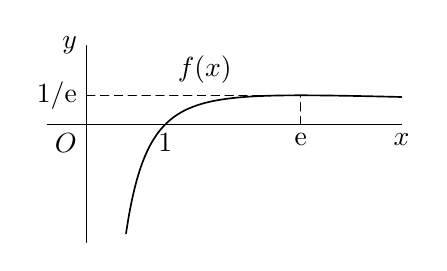
\begin{tikzpicture}[line cap=round,line join=round,scale=1]
      \draw[\myaxisarrow] (-0.5,0) -- (4,0) node[below] {$x$};
      \draw[\myaxisarrow] (0,-1.5) -- (0,1) node[left] {$y$};
      \draw[line width=0.6pt,smooth,samples=100] 
        plot[domain=0.5:4](\x,{ln(\x)/\x});
      \draw[densely dashed] (0,1/e)--(e,1/e)--(e,0);
      \draw (0,0) node[anchor=north east] {$O$}
        (0,1/e) node[left] {$1/\mathrm{e}$} 
        (1,0) node[below] {$1$}
        (e,0) node[below] {$\mathrm{e}$}
        (1.5,0.7) node {$f(x)$};
    \end{tikzpicture}\end{center}}
    在 $(\mathrm{e},+\infty)$ 上 $\searrow$.
  \endsolution
  
  \subsection{课后练习}
  \begin{exercise}
    求函数 $y=x^3 +x^2 -5x-5$ 的单调递增区间.
  \end{exercise}

  \beginsolution
    $y'=(3x+5)(x-1)$, 则 $y$ 的单调递增区间为 $\Bigl(-\infty,-\frac53\Bigr)$ 和 $(1,+\infty)$.
  \endsolution
  
  \begin{exercise}
    求函数 $f(x)=x-\ln x$ 的单调递增区间.
  \end{exercise}

  \beginsolution
    $f'(x)=\frac{x-1}x$ 且 $x>0$, 则 $f(x)$ 的单调递增区间为 $(1,+\infty)$.
  \endsolution
  
  \begin{exercise}
    求函数 $y=x-2\sin x$ 在 $(0,2\pi)$ 内的单调递增区间.
  \end{exercise}

  \beginsolution
    $y'=1-2\cos x$, 则 $y$ 的单调递增区间为 $\Bigl(\frac{\pi}3,\frac{5\pi}3\Bigr)$.
  \endsolution
  
  \begin{exercise}
    求函数 $f(x)=\frac{x-3}{\mathrm{e}^x}$ 的单调递增区间.
  \end{exercise}

  \beginsolution
    $f'(x)=\frac{4-x}{\mathrm{e}^x}$, 则 $f(x)$ 的单调递增区间为 $(-\infty,4)$.
  \endsolution
  
  \begin{exercise}
    求函数 $f(x)=x^2 -5x+2\ln x$ 的单调递增区间.
  \end{exercise}

  \beginsolution
    $f'(x)=\frac{(2x-1)(x-2)}{x}$ 且 $x>0$, 则 $f(x)$ 的单调递增区间为 $\Bigl(0,-\frac12\Bigr)$ 和 $(2,+\infty)$..
  \endsolution
  
  \begin{exercise}
    已知函数 $y=f(x)$ 的图象是图~\ref{fig-190419-2220} 中前四个图象之一, 
    且其导函数 $y=f'(x)$ 的图象如最右图所示, 则该函数的图象是\,? (填序号)
    \begin{figure}[h]
    \small
    \centering
    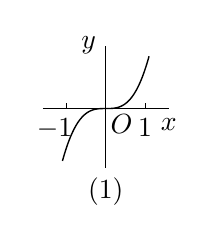
\begin{tikzpicture}[scale=0.5]
      \draw[\myaxisarrow] (-1.6,0) -- (1.6,0) node[below] {$x$};
      \draw[\myaxisarrow] (0,-1.5) -- (0,1.6) node[left] {$y$};
      \draw[line width=0.5pt,smooth,samples=100,domain=-1.1:1.1] 
        plot(\x,{(\x)^3});
      \draw (-1,0)--(-1,0.15) (1,0)--(1,0.15);
      \draw (-1.3,0) node[below] {$-1$};
      \draw (1,0) node[below] {$1$};
      \draw (0.4,-0.4) node {$O$};
      \draw (0,-2.1) node {$(1)$};
    \end{tikzpicture}\hskip 0.3cm
    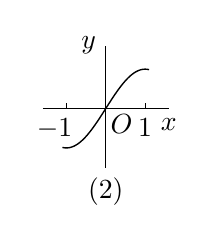
\begin{tikzpicture}[scale=0.5]
      \draw[\myaxisarrow] (-1.6,0) -- (1.6,0) node[below] {$x$};
      \draw[\myaxisarrow] (0,-1.5) -- (0,1.6) node[left] {$y$};
      \draw[line width=0.5pt,smooth,samples=100,domain=-1.1:1.1] 
        plot(\x,{sin(\x*90)});;
      \draw (-1,0)--(-1,0.15) (1,0)--(1,0.15);
      \draw (-1.3,0) node[below] {$-1$};
      \draw (1,0) node[below] {$1$};
      \draw (0.4,-0.4) node {$O$};
      \draw (0,-2.1) node {$(2)$};
    \end{tikzpicture}\hskip 0.3cm
    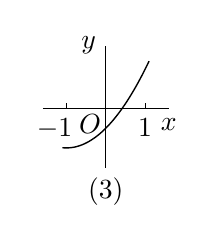
\begin{tikzpicture}[scale=0.5]
      \draw[\myaxisarrow] (-1.6,0) -- (1.6,0) node[below] {$x$};
      \draw[\myaxisarrow] (0,-1.5) -- (0,1.6) node[left] {$y$};
      \draw[line width=0.5pt,smooth,samples=100,domain=-1.1:1.1] 
        plot(\x,{2*(\x/2+1/2)^2-1});
      \draw (-1,0)--(-1,0.15) (1,0)--(1,0.15);
      \draw (-1.3,0) node[below] {$-1$};
      \draw (1,0) node[below] {$1$};
      \draw (-0.4,-0.4) node {$O$};
      \draw (0,-2.1) node {$(3)$};
    \end{tikzpicture}\hskip 0.3cm
    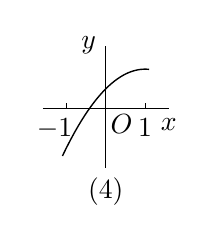
\begin{tikzpicture}[scale=0.5]
      \draw[\myaxisarrow] (-1.6,0) -- (1.6,0) node[below] {$x$};
      \draw[\myaxisarrow] (0,-1.5) -- (0,1.6) node[left] {$y$};
      \draw[line width=0.5pt,smooth,samples=100,domain=-1.1:1.1] 
        plot(\x,{1-2*(\x/2-1/2)^2});
      \draw (-1,0)--(-1,0.15) (1,0)--(1,0.15);
      \draw (-1.3,0) node[below] {$-1$};
      \draw (1,0) node[below] {$1$};
      \draw (0.4,-0.4) node {$O$};
      \draw (0,-2.1) node {$(4)$};
    \end{tikzpicture}\hskip 0.3cm
    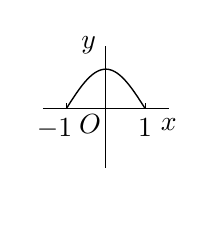
\begin{tikzpicture}[scale=0.5]
      \draw[\myaxisarrow] (-1.6,0) -- (1.6,0) node[below] {$x$};
      \draw[\myaxisarrow] (0,-1.5) -- (0,1.6) node[left] {$y$};
      \draw[line width=0.5pt,smooth,samples=100,domain=-1:1] 
        plot(\x,{cos(\x*90)});
      \draw (-1,0)--(-1,0.15) (1,0)--(1,0.15);
      \draw (-1.3,0) node[below] {$-1$};
      \draw (1,0) node[below] {$1$};
      \draw (-0.4,-0.4) node {$O$};
      \draw (0,-2.1) node {$\phantom{(4)}$};
    \end{tikzpicture}
    \caption{}\label{fig-190419-2220}
    \end{figure}
  \end{exercise}

  \beginsolution
    (2), 由 $f'(x)$ 的图象知, $f(x)$ 的图象从左往右看, 一直递增且增速变化: 慢 $\to$ 快 $\to$ 慢 (或观察切线斜率的变化).
  \endsolution
  
  \begin{exercise}
    若函数 $f(x)=x^3 +x^2 +mx+1$ 在 $\mathbb{R}$ 上单调递增, 
    求 $m$ 的取值范围.
  \end{exercise}

  \beginsolution
    $f'(x)=3x^2+2x+m\geqslant 0$ 在 $\mathbb{R}$ 上恒成立, 则 $2^2-4\cdot 3\cdot m\leqslant 0$, 所以 $m\geqslant \frac13$.
  \endsolution
  
  \begin{exercise}
    已知 $x=1$ 是函数 $f(x)=\dfrac12 x^2 -6x+a\ln x$ 的一个极值点.
    若函数 $f(x)$ 在 $(2m-1,m+1)$ 上单调递减, 求 $m$ 的取值范围.
  \end{exercise}
  
  \beginsolution
    $f'(x)= x-6-\frac{a}x$ 且 $f'(1)=0$, 所以 
    \[a=5,\quad f'(x)=\frac{(x-1)(x-5)}x,\]
    由 $x>0$ 知 $f(x)$ 在 $[1,5]$ 上 $\searrow$, 则 \[1\leqslant 2m-1< m+1\leqslant 5,\quad \text{即}\quad 1\leqslant m\leqslant 2.\]
    
    \varexercise 若题中的 $f(x)$ 在 $(2m-1,m+1)$ 上单调递增, 求 $m$ 的取值范围.
    
    由 $f'(x)=\frac{(x-1)(x-5)}x$ 和 $x>0$ 知, $f(x)$ 在 $(0,1)$ 和 $(5,+\infty)$ 上分别 $\nearrow$, 则
    \[0\leqslant 2m-1< m+1\leqslant 1\quad\text{或}\quad 5\leqslant 2m-1< m+1,\]
    均无解, 故 $m\in\varnothing$.
  \endsolution
  
%%%%%%%%%%%%%%%%%%%%%%%%%%%%%%